La composició química de l'aigua del riu Tajo va ser mesurada a través d'una anàlisis fisico-químic realitzada sobre una mostra. En aquest es va trobar una alta cantitat de partícules i ions dissolts, donant lloc a una alta conductivitat ($\sim 1000~\mu\text{S}/\cm$). També es va utilitzar un detector de germani d'alta pureza (HPGe per les sigles en anglès) per realitzar una identificació dels elements radioactius gamma presents en la mostra. En aquest es va detectar la presencia de cantitats mesurables de $\ce{^{40}K}$ i $\ce{^{226}Ra}$.

Com ja s'ha explicat, aquestes partícules han de ser elminades per dos motius. En primer lloc perquè podrien depositar-se sobre les fibres de centelleig, provocant una disminusió de l'eficiencia del detector en la detecció del triti. En segon lloc perquè aquests elements radioactius podrien ser detectats i comptabilitzats com a decaïments de triti, sobreestimant l'activitat de triti de la mostra.

Per realitzar aquesta tasca, la col·laboració TRITIUM va dissenyar un sistema de purificació de l'aigua, l'esquema del qual es mostra en la Figura \ref{fig:EsquemaSistemaAiguaUltrapura}. Aquest sistema es basa en quatre estacions succesives, composades per diversos tipos de filtres a més d'un llum ultraviolat, amb els cuals es realitza un filtratge cada volta més fi. El filtratge final aconseguit amb aquest sistema és de hasta partícules del tamany de $1~\mu\metre$, amb el cual s'aconsegueixen conductivitats de la mostra del ordre de $10~\mu\text(S)/\cm$, dos ordres de magnitud inferior a la mostra inicial.

\begin{figure}[htbp]
\centering
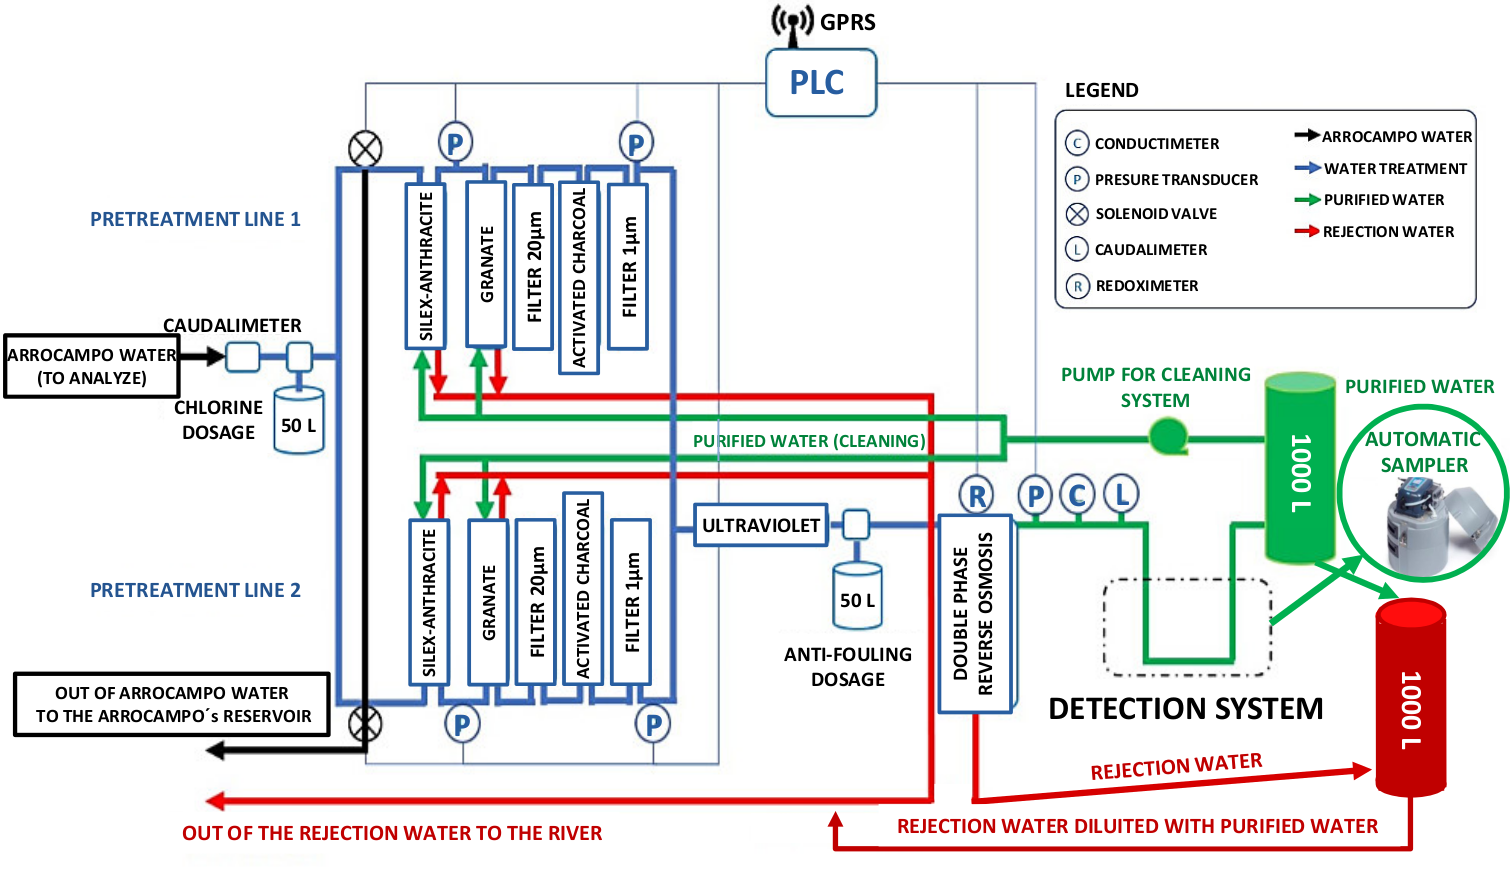
\includegraphics[scale=0.25]{12Summary/3DesignPrinciples/33UltraPureWaterSystem/SchemeUltraPureWaterSystem.png}
\caption{Esquema del sistema de purificació de l'aigua.\label{fig:EsquemaSistemaAiguaUltrapura}}
\end{figure}

Amb aquest sistema s'aconsegueix generar un total de $1.480~\meter^3/\hour$ d'aigua purificada, que sobreestima altament els requeriments del detector de triti. A més, també es va comprovar que el procés de purificació no afecta la concentració de triti de la mostra, requeriment important per a l'objectiu del projecte. Per a aquesta tasca es va utilitzar un comptador de líquid de centelleig (LSC per les sigles en anglès) per mesurar l'activitat de triti en mostres d'aigua abans i després de ser sotmeses al procés de purificació. Com es pot comprovar a la Taula \ref{tab:ValorsActivitatTriti}, l'activitat de triti de les mostres van romandre invariants al procés de purificació.

\begin{table}[htbp]
\centering{}%
\begin{tabular}{lcc}
\toprule 
Data & Antes ($\becquerel/\liter$) & Després ($\becquerel/\liter$) \tabularnewline
\midrule
\midrule 
$7/8/18$ & $24 \pm 3$ & $26 \pm 4$ \tabularnewline
$11/12/19$ & $13.2 \pm 2.1$ & $13.85 \pm 2.2$ \tabularnewline
$15/01/20$ & $30.6 \pm 4.2$ & $30 \pm 4$ \tabularnewline
\bottomrule
\end{tabular}
\caption{Mesures de l'activitat del triti de varies mostres antes i després del proces de purificació.}
\label{tab:ValorsActivitatTriti}
\end{table}

